\documentclass[11pt,letterpaper]{article}
\usepackage[margin=2.5cm]{geometry}
\usepackage[utf8]{inputenc}
\usepackage[T1]{fontenc}
\usepackage{lmodern}
\usepackage{amsmath,amssymb,amsthm,mathtools,bm}
\usepackage{enumitem}
\usepackage{booktabs}
\usepackage{tikz}
\usetikzlibrary{arrows.meta,patterns,positioning,calc}
\usepackage{pgfplots}
\pgfplotsset{compat=1.16}
\usepackage{titlesec}
\usepackage[hidelinks]{hyperref}

\setlength{\parindent}{0pt}
\setlength{\parskip}{0.5em}
\titleformat{\section}{\large\bfseries}{\thesection.}{0.6em}{}
\titleformat{\subsection}{\normalsize\bfseries}{\thesubsection.}{0.6em}{}

\theoremstyle{definition}
\newtheorem{definition}{Definition}[section]
\newtheorem{example}{Example}[section]
\newtheorem{exercise}{Exercise}[section]
\newtheorem{theorem}{Theorem}[section]
\newtheorem{remark}{Remark}[section]

\newcommand{\R}{\mathbb{R}}
\newcommand{\N}{\mathbb{N}}
\newcommand{\Z}{\mathbb{Z}}
\newcommand{\U}{\mathcal{U}}
\newcommand{\E}{\mathbb{E}}
\newcommand{\Var}{\operatorname{Var}}
\newcommand{\Cov}{\operatorname{Cov}}
\newcommand{\Normal}{\mathcal{N}}
\newcommand{\dd}{\,\mathrm{d}}
\newcommand{\T}{^{\top}}
\renewcommand{\P}{P}
\newcommand{\set}[1]{\left\{#1\right\}}
\newcommand{\given}{\mid}
\newcommand{\note}[1]{\textit{#1}}

% --- Homework exercises (tinted box) and highlighted derivation steps ---
\usepackage{tcolorbox}
\tcbuselibrary{skins,breakable}
\definecolor{hwfill}{RGB}{235,243,252}
\definecolor{hwframe}{RGB}{31,78,140}
\definecolor{newterm}{RGB}{196,78,0}
\newtcolorbox{homework}[1]{enhanced, breakable,
  colback=hwfill, colframe=hwframe, coltitle=white,
  fonttitle=\bfseries, boxrule=0.6pt, arc=2pt,
  left=6pt, right=6pt, top=4pt, bottom=4pt,
  before skip=10pt, after skip=10pt,
  title={Exercise (Homework #1)}}
\newcommand{\soln}{\par\smallskip\noindent\textbf{Solution.}\ }
% \new{...} marks what is new in a derivation step: a substituted or simplified term.
\newcommand{\new}[1]{{\color{newterm}#1}}

\title{Lecture 1: Set Theory}
\author{}\date{}

\begin{document}
\maketitle

\section*{Motivation}
Probabilistic models take into account uncertainty and deal with our imperfect knowledge of the world: our understanding of the world will always be limited by our observations.

Bayesian probabilistic models allow us to incorporate previous knowledge using conditional probabilities and Bayes' rule.

It is common sense that a model should improve in the light of new data. Bayesian models allow us to do that easily.

These features are essential in real-life applications like the Kalman filter used in robotics, GPS, radars, etc.

\textbf{Goal:} learn a model from data.

%=====================================================
\section{Review on set theory}

\begin{definition}[Set]
A \emph{set} is an unordered collection of objects, called \emph{elements} or \emph{members} of the set.
If an object $a$ is a member of a set $A$, we write $a \in A$. If $a$ is not an element of $A$, we write $a \notin A$.
\end{definition}

There are several ways to describe a set. One way is to list all members of the set, when it is possible.

\begin{example}
The set $V$ of all the vowels in the alphabet: $V = \set{a, e, i, o, u}$.
\end{example}

\begin{example}
The set $O$ of all positive odd numbers less than $10$: $O = \set{1, 3, 5, 7, 9}$.
\end{example}

\begin{example}
The elements of a set do not need to be related: $\set{2,\ i,\ +,\ \$,\ \square,\ \text{blue}}$.
\end{example}

We can also use \emph{set builder notation}: we characterize all of the elements in the set by stating their properties.
\[
O = \set{x \mid x \text{ is an odd positive integer less than } 10}
\quad\text{or}\quad
O = \set{x \in \Z^{+} \mid x \text{ is odd and } x < 10}.
\]

\textbf{Intervals:}
\begin{align*}
[a,b] &= \set{x \mid a \le x \le b}, & (a,b] &= \set{x \mid a < x \le b},\\
[a,b) &= \set{x \mid a \le x < b}, & (a,b) &= \set{x \mid a < x < b}.
\end{align*}

Sets can have other sets as members.
\begin{example}
$\set{V, O, \$, \square}$.
\end{example}

Two sets $A$ and $B$ are \emph{equal} if and only if they have the same elements. We express this as $A = B$.

\begin{example}
\begin{align*}
\set{a,b,c} &= \set{b,a,c} = \set{c,b,a},\\
\set{a,a,c,b} &= \set{a,b,c},\\
\set{b,c,a,b,c} &= \set{a,b,c}.
\end{align*}
\end{example}

\textbf{The empty set} ($\emptyset$): a special set that has no elements, also denoted $\set{\ }$.

\subsection{Conditional statements}
For propositions $p$ and $q$, the conditional statement ``if $p$, then $q$'' is denoted $p \to q$:
\begin{center}
\begin{tabular}{cc|c}
$p$ & $q$ & $p\to q$\\ \hline
T & T & T\\
T & F & F\\
F & T & T\\
F & F & T
\end{tabular}
\end{center}

\subsection{Subsets}
\begin{definition}[Subset]
A set $A$ is a \emph{subset} of $B$ if and only if every element of $A$ is also an element of $B$, denoted
\[
A \subseteq B \iff \forall x\,(x \in A \to x \in B).
\]
\end{definition}
If there exists a single element $x \in A$ such that $x \notin B$, then $A$ is not a subset of $B$: $A \not\subseteq B$.

\begin{theorem}
For every set $S$: (i) $\emptyset \subseteq S$, and (ii) $S \subseteq S$.
\end{theorem}
\begin{proof}
(i) Let $S$ be a set. To show that $\emptyset \subseteq S$, we must prove that $\forall x\,(x \in \emptyset \to x \in S)$ is true. Because $\emptyset = \set{\ }$, it follows that $x \in \emptyset$ is false. Therefore, by the truth table of $p \to q$, $x \in \emptyset \to x \in S$ is always true.

(ii) We must prove that $\forall x\,(x \in S \to x \in S)$ is true. If $x \in S$ is true, since the hypothesis and the consequence are both true, then $x \in S \to x \in S$ is always true.
\end{proof}

If $A$ is a subset of $B$ but $A \neq B$, then we write $A \subset B$ and say that $A$ is a \emph{proper subset} of $B$. For $A \subset B$, there must exist an element $x$ of $B$ that is not an element of $A$:
\[
\forall x\,(x \in A \to x \in B) \ \wedge\ \exists x\,(x \in B \wedge x \notin A).
\]
$A = B$ only if $A \subseteq B$ and $B \subseteq A$. That is,
\[
\forall x\,(x \in A \to x \in B) \ \text{ and } \ \forall x\,(x \in B \to x \in A).
\]

\begin{example}
Let $A = \set{\emptyset, \set{a}, \set{b}, \set{a,b}}$ and $B = \set{x \mid x \text{ is a subset of } \set{a,b}}$. Then $A = B$.
\end{example}

\subsection{Cardinality}
\begin{definition}[Cardinality]
If there are exactly $n$ distinct elements in a set $S$, with $n$ a nonnegative integer, we say that $S$ is a \emph{finite set} and that $n$ is the \emph{cardinality} of $S$, denoted $|S| = n$.
\end{definition}

\begin{example}
$|\emptyset| = 0$.
\end{example}
\begin{example}
$V = \set{a, e, i, o, u}$, $|V| = 5$.
\end{example}

\subsection{Power set}
\begin{definition}[Power set]
Given a set $S$, the \emph{power set} of $S$ is the set of all the subsets of $S$. It is denoted $\mathcal{P}(S)$.
\end{definition}

\begin{example}
The power set of $S = \set{a,b}$ is $\mathcal{P}(S) = \set{\emptyset, \set{a}, \set{b}, \set{a,b}}$.
\end{example}

If $|S| = n$, then $|\mathcal{P}(S)| = 2^n$. For instance:
\begin{itemize}
\item $A = \emptyset$: $\mathcal{P}(A) = \set{\emptyset} = \set{\set{\ }}$, \quad $|\mathcal{P}(A)| = 1 = 2^0$.
\item $A = \set{a}$: $\mathcal{P}(A) = \set{\set{\ }, \set{a}}$, \quad $|\mathcal{P}(A)| = 2 = 2^1$.
\item $A = \set{a,b}$: $\mathcal{P}(A) = \set{\set{\ }, \set{a}, \set{b}, \set{a,b}}$, \quad $|\mathcal{P}(A)| = 2^2$.
\item $A = \set{a,b,c}$: $\mathcal{P}(A) = \set{\set{\ }, \set{a}, \set{b}, \set{a,b}, \set{c}, \set{a,c}, \set{b,c}, \set{a,b,c}}$, \quad $|\mathcal{P}(A)| = 2^3$.
\end{itemize}

\subsection{Cartesian product}
\begin{definition}[Cartesian product]
Let $A$ and $B$ be sets. The \emph{Cartesian product} of $A$ and $B$, denoted $A \times B$, is the set of all ordered pairs $(a,b)$, where $a \in A$ and $b \in B$:
\[
A \times B = \set{(a,b) \mid a \in A \wedge b \in B}.
\]
\end{definition}

\begin{example}
Find $A \times B$ for $A = \set{a,e,i,o,u}$ and $B = \set{0,1}$:
\[
A \times B = \set{(a,0),(e,0),(i,0),(o,0),(u,0),(a,1),(e,1),(i,1),(o,1),(u,1)}.
\]
\end{example}

In general $A \times B \neq B \times A$; equality only happens when $A = B$ (for nonempty $A$, $B$).

The cardinality of the Cartesian product is $|A \times B| = |A|\,|B|$.

In general,
\begin{align*}
A_1 \times A_2 \times A_3 &= \set{(a_1,a_2,a_3) \mid a_i \in A_i,\ i = 1,2,3}, & |A_1 \times A_2 \times A_3| &= |A_1|\,|A_2|\,|A_3|,\\
A_1 \times \cdots \times A_k &= \set{(a_1,\dots,a_k) \mid a_i \in A_i,\ i = 1,\dots,k}, & |A_1 \times \cdots \times A_k| &= \prod_{i=1}^{k} |A_i|.
\end{align*}

%-----------------------------------------------------
\subsection{Set operations}

\paragraph{Universal set and Venn diagrams.}
In Venn diagrams, the universal set $\U$ is drawn as a rectangle, and a set $A$ is a perimeter enclosing some points; that is, $A$ is a set whose elements are the elements inside the perimeter. Since $\forall x\,(x \in A \to x \in \U)$, then $A \subseteq \U$.

\begin{center}
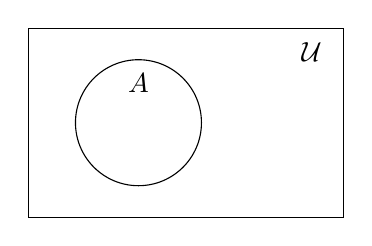
\begin{tikzpicture}
\draw (0,0) rectangle (4,2.4); \node at (3.6,2.1) {$\U$};
\draw (1.4,1.2) circle (0.8); \node at (1.4,1.7) {$A$};
\end{tikzpicture}
\end{center}

\paragraph{Union.}
For two sets $A$ and $B$, the \emph{union} $A \cup B$ is the set that contains the elements that are either in $A$ or in $B$, or in both:
\[
A \cup B = \set{x \mid x \in A \vee x \in B}.
\]
All the elements inside the perimeter of $A$ and $B$ form the set $A \cup B$.

\begin{example}
Find $A \cup B$ for $A = \set{a,b,c}$ and $B = \set{c,d}$: \ $A \cup B = \set{a,b,c,d}$.
\end{example}

\begin{center}
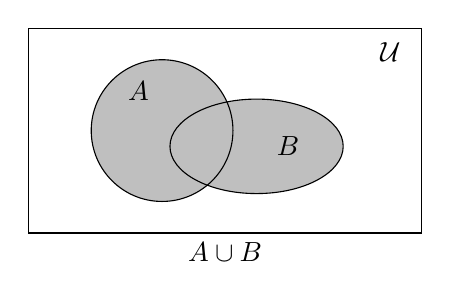
\begin{tikzpicture}
\draw (0,0) rectangle (5,2.6); \node at (4.6,2.3) {$\U$};
\fill[gray!50] (1.7,1.3) circle (0.9);
\fill[gray!50] (2.9,1.1) ellipse (1.1 and 0.6);
\draw (1.7,1.3) circle (0.9); \draw (2.9,1.1) ellipse (1.1 and 0.6);
\node at (1.4,1.8) {$A$}; \node at (3.3,1.1) {$B$};
\node[below] at (2.5,0) {$A\cup B$};
\end{tikzpicture}
\end{center}

\paragraph{Intersection.}
Let $A$ and $B$ be sets. The \emph{intersection} of the sets $A$ and $B$ is the set containing the elements in both $A$ and $B$:
\[
A \cap B = \set{x \mid x \in A \wedge x \in B}.
\]

\begin{example}
Find $A \cap B$ for $A = \set{a,b,c}$ and $B = \set{c,d}$: \ $A \cap B = \set{c}$.
\end{example}

\begin{center}
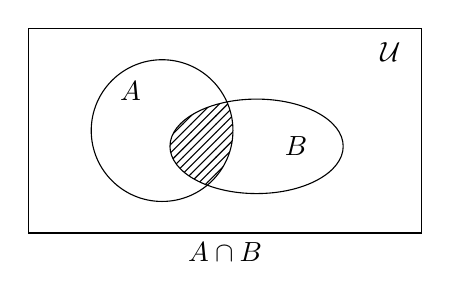
\begin{tikzpicture}
\draw (0,0) rectangle (5,2.6); \node at (4.6,2.3) {$\U$};
\begin{scope}
\clip (1.7,1.3) circle (0.9);
\fill[pattern=north east lines] (2.9,1.1) ellipse (1.1 and 0.6);
\end{scope}
\draw (1.7,1.3) circle (0.9); \draw (2.9,1.1) ellipse (1.1 and 0.6);
\node at (1.3,1.8) {$A$}; \node at (3.4,1.1) {$B$};
\node[below] at (2.5,0) {$A\cap B$};
\end{tikzpicture}
\end{center}

\paragraph{Disjoint sets.}
Two sets are called \emph{disjoint} if their intersection is the empty set: $A \cap B = \emptyset$.

\begin{center}
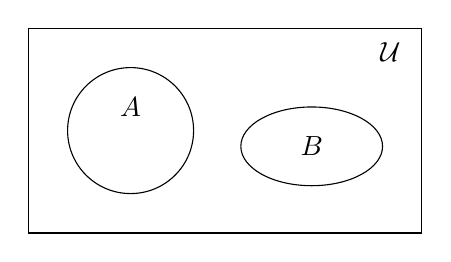
\begin{tikzpicture}
\draw (0,0) rectangle (5,2.6); \node at (4.6,2.3) {$\U$};
\draw (1.3,1.3) circle (0.8); \node at (1.3,1.6) {$A$};
\draw (3.6,1.1) ellipse (0.9 and 0.5); \node at (3.6,1.1) {$B$};
\end{tikzpicture}
\end{center}

\paragraph{Cardinality of the union.}
\[
|A \cup B| = |A| + |B| - |A \cap B|.
\]

\paragraph{Difference.}
Let $A$ and $B$ be sets. The \emph{difference} of $A$ and $B$ is defined as the set containing the elements that are in $A$ but not in $B$:
\[
A - B = A \setminus B = \set{x \mid x \in A \wedge x \notin B}.
\]

\begin{center}
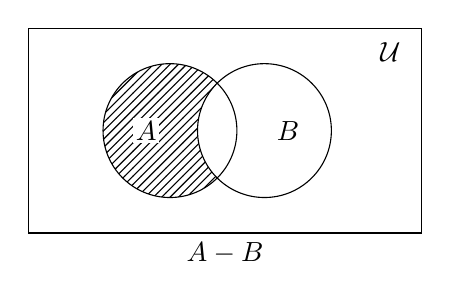
\begin{tikzpicture}
\draw (0,0) rectangle (5,2.6); \node at (4.6,2.3) {$\U$};
\fill[pattern=north east lines] (1.8,1.3) circle (0.85);
\fill[white] (3.0,1.3) circle (0.85);
\draw (1.8,1.3) circle (0.85); \draw (3.0,1.3) circle (0.85);
\node[fill=white,inner sep=1pt] at (1.5,1.3) {$A$}; \node at (3.3,1.3) {$B$};
\node[below] at (2.5,0) {$A - B$};
\end{tikzpicture}
\end{center}

\begin{example}
Let $A = \set{1,3,5}$ and $B = \set{1,2,3}$. Then $A - B = \set{5}$ and $B - A = \set{2}$.
\end{example}

\paragraph{Complement.}
Let $\U$ be the universal set. The \emph{complement} of a set $A$, denoted $A^c$ (or $\bar{A}$), is defined as
\[
A^c = \U - A = \U \setminus A = \set{x \mid x \in \U \wedge x \notin A}.
\]
It is read as the complement of $A$ with respect to $\U$.

\begin{center}
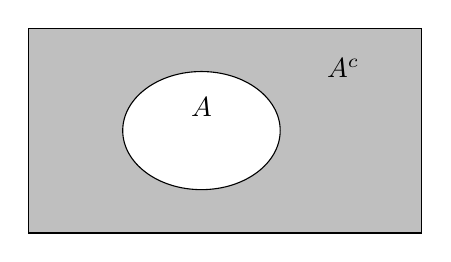
\begin{tikzpicture}
\fill[gray!50] (0,0) rectangle (5,2.6);
\fill[white] (2.2,1.3) ellipse (1.0 and 0.75);
\draw (0,0) rectangle (5,2.6); \draw (2.2,1.3) ellipse (1.0 and 0.75);
\node at (2.2,1.6) {$A$}; \node at (4.0,2.1) {$A^c$};
\end{tikzpicture}
\end{center}

\paragraph{Difference as an intersection.}
Using $A \cap C = \set{x \mid x \in A \wedge x \in C}$ and $A - B = \set{x \mid x \in A \wedge x \notin B}$: if $x \notin B$ and $B \subseteq \U$, then $x \in B^c$. Hence
\[
A - B = \set{x \mid x \in A \wedge x \in B^c} = A \cap B^c.
\]
Also,
\[
A \cap A^c = \set{x \mid x \in A \wedge x \in A^c} = \set{x \mid x \in A \wedge \neg(x \in A)} = \set{\ },
\]
since $x \in A \wedge \neg(x \in A)$ is always false.

%-----------------------------------------------------
\subsection{Set identities}

\paragraph{Double complement.} $(A^c)^c = A$. Indeed, writing $B = A^c = \set{x \mid x \in \U \wedge x \notin A}$,
\[
(A^c)^c = B^c = \set{x \mid x \in \U \wedge x \notin A^c} = \set{x \mid x \in \U \wedge x \in A} = A.
\]

\paragraph{Commutative laws.}
\[
A \cup B = B \cup A, \qquad A \cap B = B \cap A.
\]

\paragraph{Associative laws.}
\[
A \cup (B \cup C) = (A \cup B) \cup C, \qquad A \cap (B \cap C) = (A \cap B) \cap C.
\]

\paragraph{Distributive laws.}
\[
A \cup (B \cap C) = (A \cup B) \cap (A \cup C), \qquad A \cap (B \cup C) = (A \cap B) \cup (A \cap C).
\]
For the first one: with $A \cup D = \set{x \mid x \in A \vee x \in D}$ and $D = B \cap C$,
\begin{align*}
A \cup (B \cap C) &= \set{x \mid x \in A \vee (x \in B \wedge x \in C)}\\
&= \set{x \mid (x \in A \vee x \in B) \wedge (x \in A \vee x \in C)} = (A \cup B) \cap (A \cup C).
\end{align*}

\paragraph{De Morgan's laws.}
\[
(A \cap B)^c = A^c \cup B^c, \qquad (A \cup B)^c = A^c \cap B^c.
\]
For the first one, recall $D^c = \set{x \mid x \in \U \wedge x \notin D}$, where $x \notin D$ means $\neg(x \in D)$. With $D = A \cap B = \set{x \mid x \in \U \wedge (x \in A \wedge x \in B)}$,
\begin{align*}
(A \cap B)^c &= \set{x \mid x \in \U \wedge \neg(x \in A \wedge x \in B)}\\
&= \set{x \mid x \in \U \wedge (x \notin A \vee x \notin B)}\\
&= \set{x \mid (x \in \U \wedge x \notin A) \vee (x \in \U \wedge x \notin B)} = A^c \cup B^c.
\end{align*}
The same holds for $(A \cup B)^c = A^c \cap B^c$.

\paragraph{Other logical connectives.}
\[
(x \in A \Rightarrow x \in B) \equiv (x \notin A \vee x \in B), \qquad\text{i.e.}\qquad p \Rightarrow q \equiv \neg p \vee q.
\]

\begin{exercise}\leavevmode
\begin{enumerate}
\item $A \cup \emptyset = A$: \ $A \cup \emptyset = \set{x \mid x \in A \vee x \in \emptyset} = \set{x \mid x \in A} = A$, since $x \in \emptyset$ is always false.
\item $A \cap \U = \set{x \mid x \in \U \wedge x \in A}$, so $A \cap \U = A$.
\item $B \cup B^c = \set{x \mid x \in B \vee x \in B^c}$, so $B \cup B^c = \U$.
\item Use 2) and 3) to show
\[
A = A \cap \U = A \cap (B \cup B^c) = (A \cap B) \cup (A \cap B^c).
\]
Are $(A \cap B)$ and $(A \cap B^c)$ disjoint?
\end{enumerate}
\end{exercise}

\end{document}
